% -*- coding: utf-8 -*-
% -*- mode: latex -*-
%
% Template NExT Beamer Theme
%
% Autor       : Pedro Maione [pedromaionee@gmail.com]
% Copyright   : Copyright(c) 2017 NExT. Todos os direitos reservados.
% Description : Modelo de apresentação do Beamer com tema do NExT.

\documentclass[10pt,aspectratio=43,xcolor,compress]{beamer}
% --------------------------------------------------------------------------
% Pacotes e configurações
% --------------------------------------------------------------------------
\usepackage{lipsum}
\usepackage{tabularx,ragged2e}
\usepackage{booktabs}
\usepackage{listings}

\hypersetup{%
  linkcolor=nextVermelhoEscuro,
  urlcolor=magenta,
  colorlinks=true,
}

\graphicspath{%
  {./../fig/},
  {./../eps/},
}

\newcommand{\DescricaoCor}[3]{%
  \definecolor[named]{descCor}{HTML}{#1}
  \begin{tikzpicture}
    \node (quadro) [%
    rectangle,minimum width=1cm,minimum height=2cm,
    thick,draw=white,fill=descCor,] {};
  \node (texto) [right=6pt of quadro.north east, anchor=north west,] {%
    \begin{tabular}{l l}
      \textbf{HTML} & \##1\\
      \textbf{RGB} & #2\\
      \textbf{CMYK} & #3\\
    \end{tabular}
  };
\end{tikzpicture}
}

% --------------------------------------------------------------------------
% Carrega o Tema
% --------------------------------------------------------------------------
\usetheme{next}

% --------------------------------------------------------------------------
% Configurações da apresentação
% --------------------------------------------------------------------------
\title{Manual Marca}
\subtitle{NExT}
\date{\today}
\author{Pedro Maione}
\institute{\NExT}

% --------------------------------------------------------------------------
% Configuração de anotações
% --------------------------------------------------------------------------
\setbeameroption{show notes}

\begin{document}
% --------------------------------------------------------------------------
% Slide com Título
% --------------------------------------------------------------------------

\maketitle

% --------------------------------------------------------------------------
% Sumário
% --------------------------------------------------------------------------
\section*{Sumário}
\begin{frame}{Sumário}
  \tableofcontents[hideallsubsections]
\end{frame}

% --------------------------------------------------------------------------
% Conteúdo
% --------------------------------------------------------------------------
\section{Características Gerais}

\begin{frame}{Características Gerais}

O logotipo do \NExT{}  é composto pelas letras que representão a sigla no Núcleo.

\begin{figure}[!htp]
  \centering
  
\includegraphics[scale=.5]{logo-next-color}
\end{figure}

Outra opção do logotipo é a composta por símbolo e texto.

\begin{figure}[!htp]
  \centering
  \includegraphics[scale=.75]{logo-next-inline}
\end{figure}

\begin{figure}[!htp]
  \centering
  
\includegraphics[scale=.75]{logo-next-stacked}
\end{figure}


\end{frame}

\begin{frame}{Características Gerais}

Existe ainda a opção do logotipo com efeito de sombra, ilustrado abaixo.

\begin{figure}[!htp]
  \centering
  
\includegraphics[scale=1]{logo-next-shade}
\end{figure}

\end{frame}

\section{Área de não-interferência}

\begin{frame}{Área de não-interferência}

  \begin{columns}
    \begin{column}{.35\textwidth}
      Para assegurar a correta percepção, caso associado a outros elementos
      visuais, é necessário deixar uma área livre em volta do logotipo, conforme
      o diagrama ao lado.

      Sendo que o mesmo vale para o logotipo com símbolo e texto, conforme
      diagrama abaixo.
    \end{column}
    \begin{column}{.55\textwidth}
       \begin{figure}[!htp]
         \centering
         
\includegraphics[scale=1]{logo-next-clearspace}
       \end{figure}
     \end{column}
   \end{columns}
   
 \end{frame}

 \begin{frame}{Área de não-interferência}
 
\begin{figure}[!htp]
  \centering
  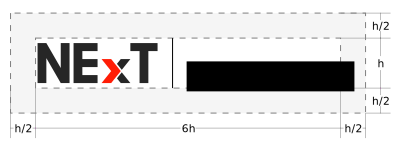
\includegraphics[scale=.75]{logo-next-inline-clearspace}
\end{figure}

\begin{figure}[!htp]
  \centering
  \includegraphics[scale=.75]{logo-next-stacked-clearspace}
\end{figure}

\end{frame}
% 

\section{Construção do logotipo}
\begin{frame}
  \frametitle{Construção do logotipo}

  \begin{columns}
    \begin{column}{.35\textwidth}
      As linhas na cor {\color[named]{magenta} magenta} indicam as proporções verticais.
    
    As linhas na cor {\color{black!30!green} verde} indicam as proporções horizontais do logotipo.

    As linhas na cor {\color{orange} laranja} representam o \emph{offset} da seta da letra ``x'' do logotipo.
    \end{column}
    \begin{column}{.65\textwidth}
      \centering
      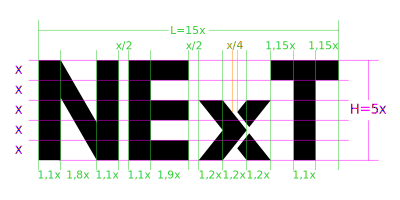
\includegraphics[scale=.75]{logo-next-grid}
     \end{column}
   \end{columns}  
\end{frame}

\begin{frame}
  \frametitle{Construção do logotipo}
  Os logotipos com símbolo e texto foram construidos como indicam os diagramas
  abaixo.

  \centering
  \includegraphics[width=\textwidth]{logo-next-inline-grid}

  \centering
  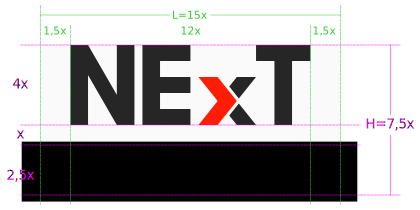
\includegraphics[scale=.75]{logo-next-stacked-grid}

\end{frame}

\section{Fontes}

\begin{frame}
  \frametitle{Fontes}

  A fonte utilizado para o logotipo foi a \emph{League Spartan}, obtida no
  \href{https://www.fontsquirrel.com/fonts/league-spartan}{Font Squirrel}, e
  está definida sob a licensa \emph{SIL Open Font License v1.10}. No entanto,
  foi necessário adequar ao grid, gerando uma variação em relação à fonte
  original.
  
  \centering
  \includegraphics[width=.8\textwidth]{league-spartan_720x300.png}

\end{frame}
% 

\begin{frame}
  \frametitle{Fontes}
  \begin{columns}
    \begin{column}{.35\textwidth}
      Para ilustrar as alterações realizadas em relação à fonte original temos a imagem ao lado.
    \end{column}
    \begin{column}{.55\textwidth}
      \centering
    
\includegraphics[scale=.75]{logo-next-comparacao}
     \end{column}
   \end{columns}

\end{frame}

\begin{frame}
  \frametitle{Fontes}
  Para os logotipos com símbolo e texto, é utilizado a fonte \emph{Roboto},
  disponível no \href{https://fonts.google.com/specimen/Roboto}{Google~Fonts}.

  \centering
  \includegraphics[width=.8\textwidth]{roboto-720x300.png}

\end{frame}

\section{Padrões Cromáticos}

\begin{frame}
  \frametitle{Cores Primárias}

  O símbolo do \NExT{} é composto por duas cores principais.


  \begin{center}
    \DescricaoCor{FF1D06}{255, 29, 6}{0, 89, 98, 0}
    \DescricaoCor{262626}{38, 38, 38}{0, 0, 0, 85}
  \end{center}

\end{frame}

\begin{frame}
  \frametitle{Cores Secundárias}

  \DescricaoCor{FF9206}{255, 146, 6}{0, 43, 98, 0}
  \vfill
  \DescricaoCor{0E65A3}{14, 101, 163}{91, 38, 0, 36}
  \vfill
  \DescricaoCor{04C02E}{4, 192, 46}{98, 0, 76, 25}

\end{frame}

\begin{frame}
  \frametitle{Variações}

  Para obter uma paleta de cores com as variações, utilize os links abaixo:

  \begin{itemize}
  \item \href{http://paletton.com/\#uid=7040D0kvjvXojH8rfABuGpcuRk9}{Paleta de cores}
  \item \href{http://paletton.com/\#uid=1000D0k004M0dcY0dcY5o003H00}{Paleta de escala de cinza}
  \end{itemize}

  \noindent
  Para obtenção das paletas de cores, foi utilizado a ferramenta
  \href{http://paletton.com}{http://paletton.com}.

    \centering
    Paleta de cores completa.
    \includegraphics[scale=.75]{paleta-cores-escala}
\end{frame}

\begin{frame}
  \frametitle{Escala de Redução}

  O logotipo nunca deve ser reduzido a um tamanho menor que os indicados
  abaixo. Em cada diagrama está representado as dimensoẽs mínimas para apicações
  eletrônicas em \emph{pixels} e para impressão e publicação em
  \emph{milimetros}

  {\bfseries Atenção: Os valores entre parênteses, na cor {\color{magenta}
      magenta} não representam a conversão de \emph{pixels} para milimetros.}

  \vfill
  \centering
  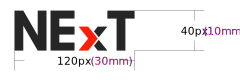
\includegraphics[scale=1]{logo-next-minimo}

\end{frame}

\begin{frame}
  \frametitle{Escala de Redução}

  \vfill
  \centering
  \includegraphics[scale=1]{logo-next-inline-minimo}
  \vfill
  \centering
  \includegraphics[scale=1]{logo-next-stacked-minimo}
  \vfill
  
\end{frame}

\section{Variantes do Logotipo}

\begin{frame}
  \frametitle{Variantes do Logotipo}

  \noindent Versões colorida, positivo e negativo

  \centering
  \includegraphics[scale=1]{logo-next-color-variacoes-01}

  \noindent Versões monocromáticas, positivo e negativo

  \centering
  \includegraphics[scale=1]{logo-next-color-variacoes-02}

  \noindent Versões coloridas com sombra, positivo e negativo

  \centering
  
\includegraphics[scale=1]{logo-next-color-variacoes-03}

\end{frame}

\begin{frame}
  \frametitle{Outras variações do logotipo}

  Podem ser obtidos outras variantes do logotipo, com a utilização dos logotipos
  com símbolo e texto, em linha ou empilhado, seguindo as orientações acima. Por
  exemplo:

  \vfill
  \centering
  
\includegraphics[scale=1]{logo-next-color-variacoes-04}
  \vfill

\end{frame}

\end{document}

% Local Variables:
% TeX-engine: xetex
% End:
